\documentclass[a4paper,12pt]{article}

% Packages
\usepackage{float}
\usepackage[utf8]{inputenc}
\usepackage{fancyhdr}
\usepackage[left = 0.6 in, right = 0.6 in, top = 1 in, bottom = 1 in, headsep = 0.5 in]{geometry}
\usepackage[normalem]{ulem}
\usepackage{enumerate}
\usepackage{pgfplots}
\usepackage{titling}
\pgfplotsset{width=8cm,compat=1.9}
\usepackage{stackengine}
\usepackage{algorithm}
\usepackage[noend]{algpseudocode}
%\pagenumbering{gobble} 
\usepackage{amsmath} % add [fleqn] before {amsmath} to left center
\usepackage{amssymb}
\usepackage[T1]{fontenc}
\usepackage{fancybox}
\usepackage{longtable}
\usepackage{tikz}
\usepackage{subcaption}
\usepackage{chngcntr}


\DeclareMathOperator*{\argmax}{arg\,max}
\DeclareMathOperator*{\argmin}{arg\,min}

\hfuzz = 100pt

% For heaps
\tikzset{
  heap/.style={
    every node/.style={circle,draw},
    level 1/.style={sibling distance=30mm},
    level 2/.style={sibling distance=15mm}
  }
}


%%% Horizontal Line Command
\makeatletter
  \newcommand*\variableheghtrulefill[1][.4\p@]{%
    \leavevmode
    \leaders \hrule \@height #1\relax \hfill
    \null
  }
\makeatother
%%%

%%% Algorithm commands
\algblock{Input}{EndInput}
\algnotext{EndInput}
\algblock{Output}{EndOutput}
\algnotext{EndOutput}
\newcommand{\Desc}[2]{\State \makebox[3em][l]{#1}#2}
%%%

% %%% Header & Footer
% \fancyhf{}
% \renewcommand{\footrulewidth}{0.1mm}
% \fancyhead[L]{Matteo Esposito}
% \fancyhead[R]{COMP 352-X}
% \fancyfoot[R]{\thepage}

% \pagestyle{fancy}
% %%%

% Code formatting
\newcommand{\code}[1]{\texttt{#1}}

\renewcommand\maketitlehooka{\null\mbox{}\vfill}
\renewcommand\maketitlehookd{\vfill\null}

\setlength{\abovedisplayskip}{2pt}
\setlength{\belowdisplayskip}{3pt}

% Custom settings
\setlength{\parskip}{0.75em}  % Paragraph spacing
\setcounter{section}{-1} % Page numbers to start on page 1
\setlength\parindent{0pt} % Remove indenting from entire file
\def\layersep{2.5cm}

\title{
{STAT 497 - Final Project} \\
{\large Concordia University} \\
}
\date{}

%--------------------------------------------------------------------------%

\begin{document}

\begin{titlingpage}
  \maketitle
  \centering
  \vfill
  {\large{Bakr Abbas, Matthew Liu, Frederic Siino}} \par
  {\large{Day Month Year}}
\end{titlingpage}

\newpage

\section{To do list}

\begin{itemize}
  \item Add footnotes
  \item Add links (to Jiang et al. and Sutton and Barto)
  \item Add references
  \item Add grid search results
  \item Add figures for policy gradient analysis
  \item Add function description for policy gradient
  \item Add conclusion
  \item Determine if extra analysis should be added
  \item Add table of contents
  \item Review report
\end{itemize}

\newpage

\section{Introduction}
One of the main challenges of managing a portfolio or a fund, is the decision process of how to allocate investment resources to each assets. The goal is to maximize returns but also to take into account the variability of the market. The strategy to put all the fund in the most profitable asset could be beneficial in the short run. However, the possibility of that one asset crashing in value is larger than the possibility of multiple assets crashing in value. A portfolio manager should thus diversify its portfolio by investing in multiple assets. This management strategy applies to various class of assets (stocks, real estates, bonds,currencies, etc.). Some markets are more volatile than others due to various reasons. For instances, real estates is much less liquid, hence less volatile than currencies. Currency market has a very high volume of trading. 
 \\

Cryptocurrencies are decentralized digital assets that behave as an alternative to government issued money. They are being introduced into most investment portfolios. This paper addresses the challenges of managing five different cryptocurrencies with Bitcoin (BTC) being the benchmark. Meaning that the four other currencies are quantified as the price relative to BTC.  Different reinforcement learning methods will be used to manage and optimize the weights assigned to each asset in the portfolio. The first three methods will be based on the contextual bandits model. The final method will be based on a policy gradient model. A more realistic model would also take transaction costs into account, but this will be overlooked for simplicity. \\

A previous research paper (Jiang, Xu, Liang, 2017) has been published on this exact topic based on a framework consisting of Ensemble of Identical Independent Evaluators (EIIE), a Portfolio-Vector Memory (PVM), an Online Stochastic Batch Learning (OSBL) scheme and a fully exploiting strategy. The actions were determined using a policy gradient method and the tested evaluators were a Convolutional Neural Network (CNN), a Recurrent Neural Network (RNN) and a Long Short-Term Memory Network (LSTM). Experiments were run with a trading period of 30 minutes and the RL framework was observed to behave far better than other optimization frameworks in the test period of 2017 but inferior to some frameworks in the test period of 2018. \\

In this project, we opt for a much simpler approach, relying instead on an action preference function and a policy gradient when framing the task as a contextual bandits problem. We do however borrow some aspects of Jiang, Xu and Liang such as definitions for states and returns. \\

\section{Problem description}
In this project, the environment is solely dictated by the data of the historic prices of all cryptocurrencies relative to BTC. In the experiments, a trading period of $T = 120$ minutes is used, and we only consider the closing prices of each period (which are equivalent to the opening prices of the next period). In addition, the experiments rely on two key assumptions (Jiang, Xu, Liang, 2017):

\begin{itemize}
  \item Instant liquidity: The liquidity of the market allows each trade to be carried out immediately at the price listed when the order is placed.
  \item No market impact: The capital invested by the agent is so insignificant as to have no impact on the market.
\end{itemize}

This means that the sequence of states and transition probabilities are already predefined based on the data at hand. In particular, we define a price relative vector $y_t$ of the $t$th trading period like Jiang, Xu and Liang, namely:
\begin{equation}
y_t := v_t \oslash v_{t-1} = \bigg(1,\frac{v_{2,t}}{v_{2,t-1}}, …,\frac{v_{m-1,t}}{v_{m-1,t-1}}, \frac{v_{m,t}}{v_{m,t-1}}\bigg)^T
\end{equation}
where $v_{t,i}$ denotes the closing price of the $i$th asset in the $t$th trading period. Note here that asset 1 and thus $v_{t,1}$ is always equal to 1. This is because the relative prices $v_{t,i}$ are relative to the first asset (in our case, BTC), also known as the cash. This price relative vector can then be used to calculate the reward, defined in general as 
\begin{equation}
r_t = y_t \cdot w_{t-1}
\end{equation}
where $w_{t-1}$ is the portfolio weight vector at time $t-1$. This reward is effectively the change in portfolio value for period $t$. The action $a_t$ at time $t$ is the portfolio weight vector $w_t$, where the $i$th element is the proportion of asset $i$ in the portfolio.
\begin{equation}
a_t := w_t
\end{equation}
The goal of the agent is then to maximize the growth rate (or cumulative return) $r_t$ of the portfolio over the experimental time frame. \\

In addition, we also define a state vector $S_T := (s_{1,T},...,s_{m,T})$ where $s_{i,T}$ denotes the state of the previous price changes of asset $i$ at time $T$. Namely,
\begin{equation}
s_{i,T} = \sum_{t=T-n}^{t=T} \gamma^t y_{i,t}
\end{equation}
where $y_{i,t}$ is the $i$th element of the previously defined price relative vector $y_t$, $\gamma$ is a discount factor and $n$ is the size of the history we consider. As such the state is a vector of $n$-step backward relative price changes for each asset discounted by a rate gamma. \\

Thus, based on the environment and problem definition, we have 
\begin{equation}
p(s_{t+1} | s_t,a) := Pr[S_{t+1}=s_{t+1} | S_t=s_t,A_t=a] = 1 \; \forall a \in A
\end{equation}
for the deterministic sequence of states
$$S_1,S_1,...,S_{T-n}$$
which follows since the sequence $y_1,y_2,...,y_T$ is determined by the data. \\

For the sake of simplicity, an additional assumption that there are no transaction fees is added. Thus the focus turns to wether or not the agent is able to learn the optimal re-weighting of the portfolio given the state at each time, i.e. the agent must identify promising assets. The question of transaction fees and practicality will be judged in a seperate analysis. \\

Lastly, since we let the agent run through all the available data when conducting an experiment, the problem becomes an episodic task where $t=1,...,T-n$ and $T$ is the number of trading periods in our data set. Note here that $t$ ends at $t=T-n$ since the window of the first $n$ price changes needs to be considered as the starting state $S_1$, therefore reducing the number of states from $T$ to $T-n$. In practice however, the problem is a continuing task since the agent is tasked to a manage a portfolio forever.

\section{Implementations and Analyses}

\subsection{Method 1}

\subsubsection{Implementation}
Method 1 is an ad-hoc method based on the contextual bandits problem. The portfolio allocation optimization problem is reframed as a k-armed bandits problem where we have one arm for each asset in the portfolio (including cash). The action preference method is used, where 
$$H_t(a), \; a = 1,...,k$$
are the action preferences for all k assets. However, a slight modification is done when defining actions and updating the preference functions. When computing probabilities of chosing a given action, we define $\pi_t(a|S_t)$ as
\begin{equation}
\pi_t (a|S_t) := Pr[A_t=a | S_t,R_1,...,R_{t-1}] = \frac{e^{H_t(a) S_{a,t}}}{\sum_{b=1}^{k} e^{H_t(b) S_{b,t}}}, \; a=1,...,k
\end{equation}
where the previously defined state vector $S_t$ from equation (4) is included due to the contextual nature of the problem. The $n$-size history of discounted price changes represented by $S_t$ will thus change the probabilities of each asset based on whether or not their prices are observed to have declined or increased in the past $n$ periods (uptrends increase preference, and downtrends decrease preference). Following the standard contextual bandits framework, this leads to the action at time $t$ of
\begin{equation}
A_t = \argmax_a \pi_t(a|S_t)
\end{equation}
In the form of a portfolio weight vector, $A_t = w_t$ is a $k$-length vector where the $A_t$th co-ordinate is 1 and all other co-ordinates are 0. This means that rewards are
\begin{equation}
R_{t+1} := y_{t+1} \cdot A_t = y_{t+1,A_t}
\end{equation}
i.e., the relative price change of asset $A_t$. The problem then reduces to a simple contextual bandits problem where one and only one arm is pulled by the agent at each time steps. \par
However, in the ad-hoc method the actual action taken by the agent at time $t$ is the vector of contextual preference values, i.e. 
\begin{equation}
A_t' = (\pi_t(1|S_t),\pi_t(2|S_t),...,\pi_t(k|S_t))^T
\end{equation}
Since all $\pi_t(k|S_t)$'s sum to 1, this is a valid portfolio weight vector, and we can set $A_t' = w_t$. The rewards are then computed as 
\begin{equation}
R_{t+1}' :=  y_{t+1} \cdot A_t'
\end{equation}
and the preference functions are updated based on $R_t'$ as follows:
\begin{equation}
H_{t+1}(A_t) = H_t(A_t) + \alpha (R_t' - \bar{R_t})(1 - \pi_t(A_t))
\end{equation}
\begin{equation}
H_{t+1}(a) = H_t(a) - \alpha (R_t' - \bar{R_t})\pi_t(a), \; a \neq A_t
\end{equation}
where $\pi_t(a)$ represents the non-contextual policy 
\begin{equation}
\pi_t (a) := Pr[A_t=a | R_1,...,R_{t-1}] = \frac{e^{H_t(a)}}{\sum_{b=1}^{k} e^{H_t(b)}}, \; a=1,...,k
\end{equation} \\
Intuitively, this method relies on the simplfying assumption that rewards produced by actions $A_t'$ is a good enough approximation of rewards produced by actions $A_t$. In other words, 
$$E[R_t' | S_t] \approx E[R_t | S_t]$$
In reality however, we can predict that this is far from the case (hence the ad-hoc nature of this method). It is safe to assume that computing the returns of a preference vector of assets is not the same as computing the total one-step return of the single most preferred asset. Nevertheless, the ad-hoc method provides a straightforward way to implement an algorithm learning to optimize a portfolio of assets since the softmax produces valid actions that represent the preference of the agent at time $t$ based on $S_t$. However, the actual rewards used to update the preference function is only a weak approximation of the actual reward $R_t$ defined in equation (8).

The function used to simulate a single episode of method 1 is \code{simulate\_contextual1} and the parameters are as follows:
\begin{itemize}
  \item \code{n\_curren}: The number of currencies in the problem including cash (5 for this project)
  \item \code{n\_steps}: The number of timesteps $T$ in the episode. To use all available data set \code{n\_steps = nrow(data)}
  \item \code{alpha}: Learning rate $\alpha$ when updating action preference function (as defined above)
  \item \code{window\_size}: Size of historic prices to consider when computing $S_t$ (\code{window\_size} corresponds to the value of $n$)
  \item \code{discount}: Discount factor of previous relative price changes when computing $S_t$ (\code{discount} corresponds to the value of $\gamma$)
  \item \code{data}: data that is used to run experiments
\end{itemize}

\subsubsection{Analysis}
Using this ad-hoc method, the agent consistently beats the market returns even when the learning rate and the window size. The reason behind this is due to one of the currencies, XRP, having a very steep increase in value (add footnote to refer to xrp spike). This increase causes a shift in the agent’s preference to heavily to invest more in XRP during this spike. The action preferences for method 1 have a higher variance than method 2, which is noticable visually when looking at the graph of the preferences of each currency. 

A grid search was conducted to find an optimal window size and alpha combination that would result in a higher agent return (add footnote to results). Combinations from alpha values ranging from 0.1 to 0.4, and window sizes ranging from 6 to 12. It was found that the best combination in this range was an alpha of 0.4 \& a window size of 12, as the agent experiences a return of about 137\% while the market return was roughly 85\%. The larger alpha will cause the agent to prefer XRP even more during it’s spike, which is between time step 2000 \& 4000.
This method does accomplish our main goal, which is to beat the market.

\begin{figure}[h!]
  \centering
  \begin{subfigure}[b]{0.4\linewidth}
    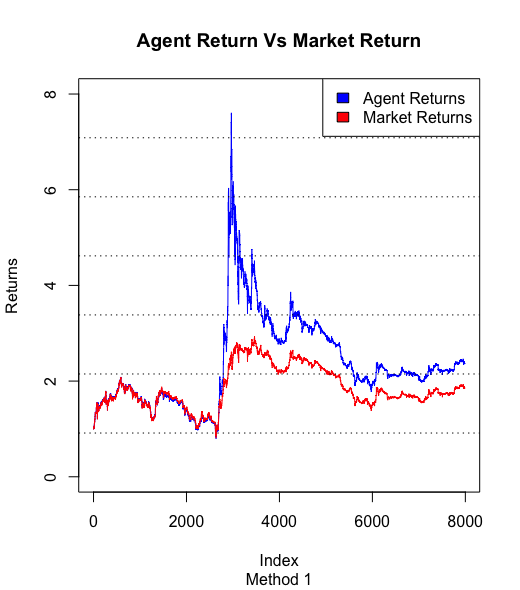
\includegraphics[width=\linewidth]{figures/agt_vs_mkt1.png}
  \end{subfigure}
  \begin{subfigure}[b]{0.4\linewidth}
    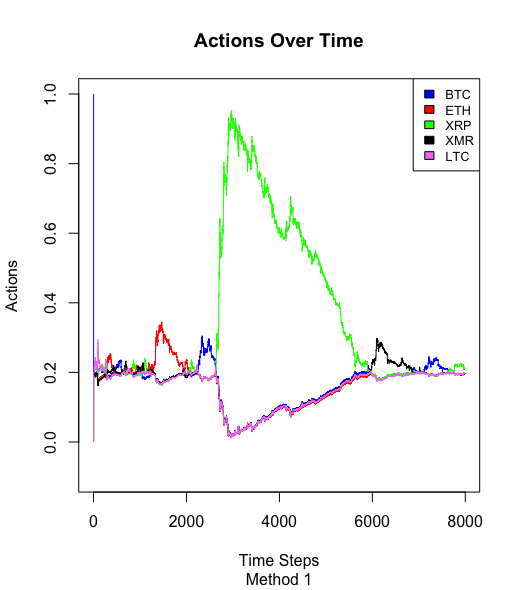
\includegraphics[width=\linewidth]{figures/actions1.png}
  \end{subfigure}
  \caption{Agent performance and agent actions over time (method 1)}
  \label{fig:method1}
\end{figure}

\subsection{Method 2}

\subsubsection{Implementation}
Method 2 is another preference function method that takes advantage of the fact that actions carried out by our agent do not affect rewards and transition probabilities. As such it is possible to sample many different actions at each timestep and observe rewards that follow had the agent taken that action. \\
Again we define a contextual policy function $\pi_t (a|S_t)$ and a normal policy function $\pi_t (a)$ from equations (6) and (13) respectively.
We also define a new reward vector $R_{t}^{All}$ where
\begin{equation}
R_{t}^{All} := y_t
\end{equation}
and $y_t$ is the previously defined relative price change vector in (1). This is because the price relative vector is a vector of rewards where the $a$th element in $y_t$ is the reward  resulting from the agent investing all its capital into asset $a$. This new reward vector $R_{t}^{All}$ becomes the basis of the action preference updates. In particular, we use a new average reward $\bar{R_t}^{All}$ as
\begin{equation}
\bar{R_t}^{All} := \frac{1}{5t} \sum_{T=1}^{t} \sum_{a=1}^{5} R_{T,a}^{All}
\end{equation}
where we sum from $a=1$ to 5 since there are 5 assets in the portfolio and $R_{T,a}^{All}$ denotes the $a$th element of the vector $R_{T}^{All}$. In other words, $\bar{R_t}^{All}$ computes the mean of the concatenation of vectors
\begin{equation}
(R_1^{All},R_2^{All},...,R_t^{All})^T
\end{equation} \\
Intuitively, this means that the average reward $\bar{R_t}^{All}$ becomes the market average at time $t$. We can then update preferences as follows:
\begin{equation}
H_{t+1}(a) = H_t(a) + \alpha (R_{t,a}^{All} - \bar{R_t}^{All})(1 - \pi_t(a)), \; a = 1,...,5
\end{equation}
In other words, the preference for each asset is updated according to the observed reward for that asset and the average of all previous rewards, effectively making the method rely on 5 different independent preference functions that monitor one asset each. Like the ad-hoc method, the action taken by the agent is the same as in (9),
$$A_t' = (\pi_t(1|S_t),\pi_t(2|S_t),...,\pi_t(5|S_t))^T$$ 
and the reward used to measure its performance is once again
$$R_{t+1}' :=  y_{t+1} \cdot A_t'$$ \\
However, this time, none of the agent rewards $R_{t+1}'$ are used to update the preference functions $H_t(a)$. This means that the update functions for each $H_t(a)$ are valid since the sequence of preference functions 
$$H_1(a),H_2(a),...,H_t(a)$$
represents the preference values for an agent that invests all its capital into asset $a$ during each trading period (compared to the baseline $\bar{R_t}^{All}$ equal to the market average). The agent's action $A_t'$ is therefore a softmax vector that represents the relative preferences of each indenpendent evaluator. We can predict that method 2's rewards are much less volatile than method 1's since the estimates of each asset are continuously updated at each time step. As such the preferences should also contain less variance.

The function used to simulate a single episode of method 2 is \code{simulate\_contextual2} and the parameters are as follows:
\begin{itemize}
  \item \code{n\_curren}: The number of currencies in the problem including cash (5 for this project)
  \item \code{n\_steps}: The number of timesteps $T$ in the episode. To use all available data set \code{n\_steps = nrow(data)}
  \item \code{alpha}: Learning rate $\alpha$ when updating action preference function (as defined above)
  \item \code{window\_size}: Size of historic prices to consider when computing $S_t$ (\code{window\_size} corresponds to the value of $n$)
  \item \code{discount}: Discount factor of previous relative price changes when computing $S_t$ (\code{discount} corresponds to the value of $\gamma$)
  \item \code{data}: data that is used to run experiments
\end{itemize}

\subsubsection{Analysis}
Using this method the agent follows the market, the returns are slightly below the market but it experiences positive returns (63.8\%). The preferences in method 2 varry a lot less than method 1 since the preferences are updated as if each “arm” was pulled (as opposed to the action being the argmax of the softmax output given the state). The largest increase in preference was observed when XRP had a large spike as discussed previously. But the effects were not as drastic as the previous method since the preferences are updated more uniformly.
A grid search was once again used to find the optimal parameters as in method one (add reference to grid search results here). In addition, the same range of values were used for alpha and window size. The outcome was that the lowest learning rate would result in the highest return as well as the lowest window size. 
The main goal of this modeling is to train an agent to beat the market, but in this method it has failed to do so. 

\begin{figure}[h!]
  \centering
  \begin{subfigure}[b]{0.4\linewidth}
    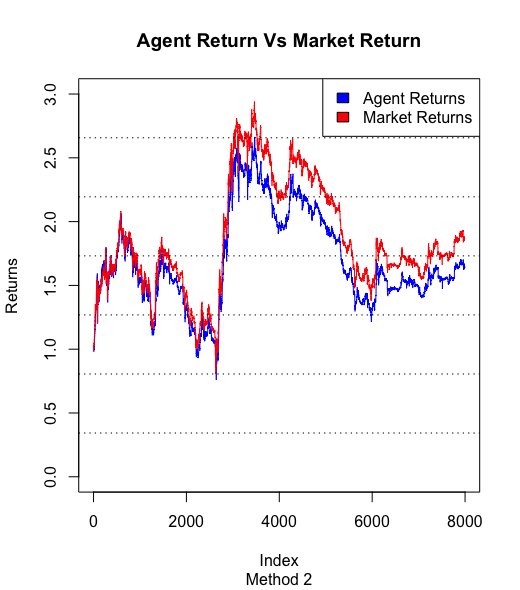
\includegraphics[width=\linewidth]{figures/agt_vs_mkt2.png}
  \end{subfigure}
  \begin{subfigure}[b]{0.4\linewidth}
    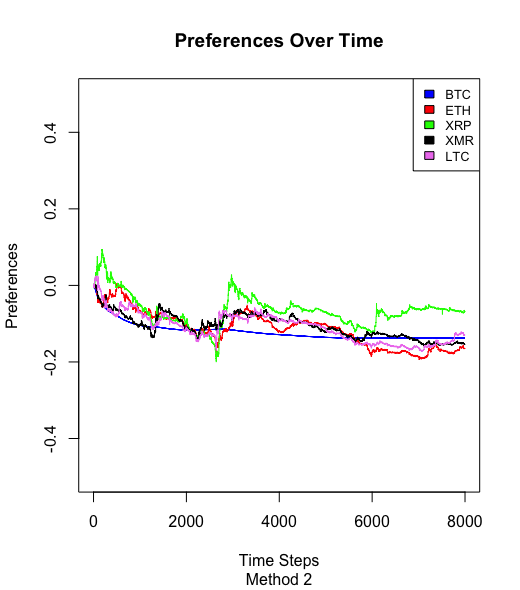
\includegraphics[width=\linewidth]{figures/prefs2.png}
  \end{subfigure}
  \caption{Agent performance and agent preferences over time (method 2)}
  \label{fig:method2}
\end{figure}

\subsection{Method 3}

\subsubsection{Implementation}
Method 3 (dubbed the "all-or-nothing" method" is the original contextual bandits with action preference function method outlined in the section for method 1. We use the softmax and the previously defined state vector $S_t$ to form our action probabilities $\pi_t (a|S_t)$ and $\pi_t (a)$ ((6) and (13)).
The action taken by the agent is then from (7)
$$A_t = \argmax_a \pi_t(a|S_t)$$
More formally, when computing the reward, the action $A_t$ becomes the standard basis vector $w_t$ where 
\begin{equation}
w_t := e_{A_t}
\end{equation}
and the vectors $e$ are defined as 
$$e_1 := (1,0,0,0,0)^T, \; e_2 := (0,1,0,0,0)^T, \; e_3 := (0,0,1,0,0)^T, \; e_4 := (0,0,0,1,0)^T, e_5 := (0,0,0,0,1)^T$$
when the number of assets $k=5$. \par
This leads to the aforementioned definition of the reward (8),
$$R_{t+1} := y_{t+1} \cdot A_t = y_{t+1,A_t}$$
which is the relative price change of asset $A_t$. The preference can now be correctly updated as 
\begin{equation}
H_{t+1}(A_t) = H_t(A_t) + \alpha (R_t - \bar{R_t})(1 - \pi_t(A_t))
\end{equation}
\begin{equation}
H_{t+1}(a) = H_t(a) - \alpha (R_t - \bar{R_t})\pi_t(a), \; a \neq A_t
\end{equation} 
which differ from (11) and (12) since we are now using the correct observations $R_t$ instead of $R_t'$. \par
The all-or-nothing method is essentially the simplest algorithm for tackling the portfolio optimization problem, since it is equivalent to the k-armed contextual bandits framework where we can assume rewards for each arm are non-stationary and we only pull one and one arm only at each time step. In practice, this means that the agent reallocates all the capital of the portfolio into one currency during each trading period based on its preference function, which can lead to extremely volatile rewards as well as large transaction costs (if such fees were considered). In addition, since the we assume non-stationarity, an epsilon greedy strategy is asseumed.

The function used to simulate a single episode of method 3 is \code{simulate\_contextual3} and the parameters are as follows:
\begin{itemize}
  \item \code{n\_curren}: The number of currencies in the problem including cash (5 for this project)
  \item \code{n\_steps}: The number of timesteps $T$ in the episode. To use all available data set \code{n\_steps = nrow(data)}
  \item \code{alpha}: Learning rate $\alpha$ when updating action preference function (as defined above)
  \item \code{window\_size}: Size of historic prices to consider when computing $S_t$ (\code{window\_size} corresponds to the value of $n$)
  \item \code{discount}: Discount factor of previous relative price changes when computing $S_t$ (\code{discount} corresponds to the value of $\gamma$)
  \item \code{epsilon}: $\epsilon$ value (for epsilon greedy)
  \item \code{data}: data that is used to run experiments
\end{itemize}

\newpage

\subsubsection{Analysis}
This is the only method that will have an element of randomness, as it uses an epsilon greedy approach. In practice the transaction costs involved in this method would be very high when compared to the other method.The “all or nothing” method  experiences the worst returns when compared to the other Contextual Bandit methods. It is the only the method that actually experiences negative returns, but this changes drastically when the seed is changed. The only way this method can perform better is if it is able to identify the currency that will beat the market at each time step, but this is not possible given the simplicity of the model.
The grid search was not conducted for this method since the seed changes what the returns will be. 
This method does not perform well. The non-stationary nature of the problem forces the agent to continuously explore, and thus there is no true convergence. 

\begin{figure}[h!]
  \centering
  \begin{subfigure}[b]{0.4\linewidth}
    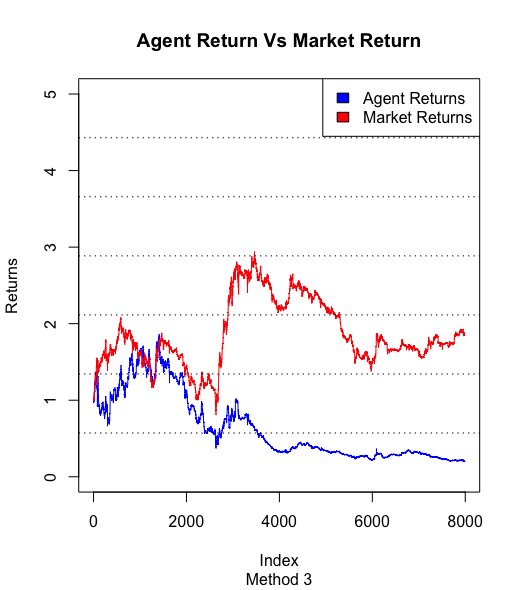
\includegraphics[width=\linewidth]{figures/agt_vs_mkt3.png}
  \end{subfigure}
  \begin{subfigure}[b]{0.4\linewidth}
    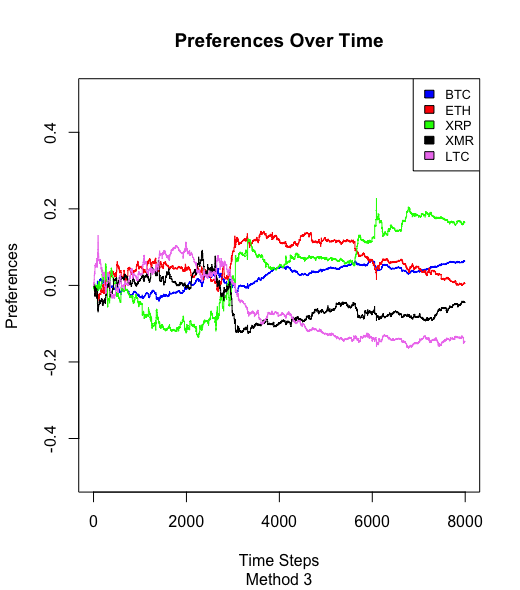
\includegraphics[width=\linewidth]{figures/prefs3.png}
  \end{subfigure}
  \caption{Agent performance and agent preferences over time (method 3)}
  \label{fig:method3}
\end{figure}

\subsubsection{Contextual bandits comparison}
When comparing all contextual bandits methods, it can be seen that the ad-hoc method beats all the other methods as well as outperforming the market. As discussed earlier this is mainly due to the spike in XRP and how the agent decides to heavily invest in it. When only using the data past the spike, the returns from all the methods are very close to each other. It should be noted that method 3 should not be compared it’s previous return since there is randomness and the agent would not make the same decisions it made initially. Method 1 is almost invisible since it has almost the same returns as the market.

\begin{figure}[h!]
  \centering
  \begin{subfigure}[b]{0.4\linewidth}
    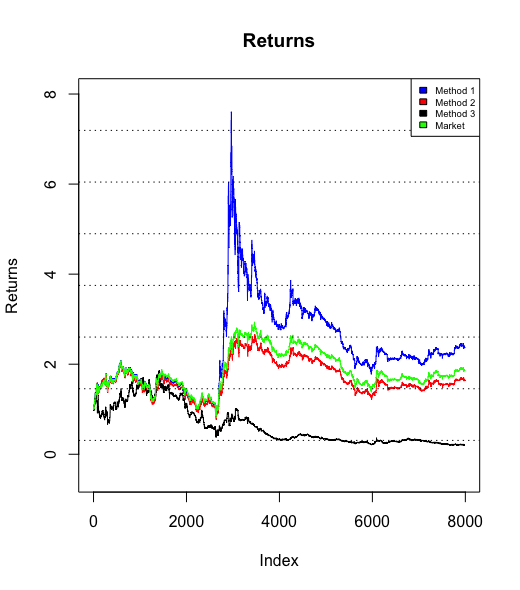
\includegraphics[width=\linewidth]{figures/returns.png}
  \end{subfigure}
  \begin{subfigure}[b]{0.4\linewidth}
    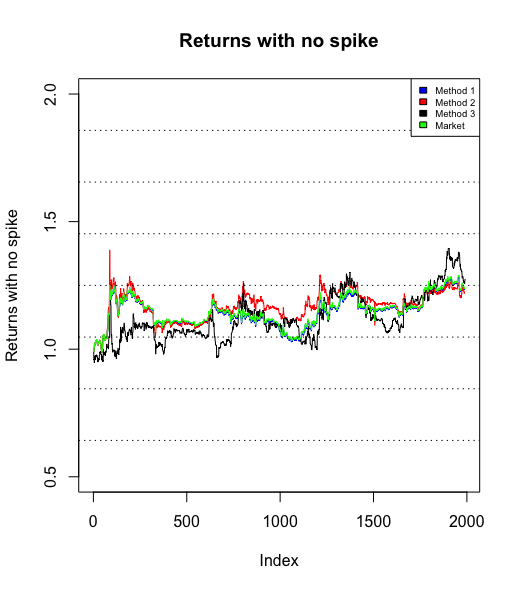
\includegraphics[width=\linewidth]{figures/returns_no_spike.png}
  \end{subfigure}
  \caption{Comparison of performance of first 3 methods (with and without spike)}
  \label{fig:comparison}
\end{figure}

\subsection{Method 4}

\subsubsection{Implementation}
Similarly to method 1, method 4 is also an ad hoc method based on policy gradient method. The portfolio allocation problem is framed as a k-armed bandits problem where the actions are the five cryptocurrencies (including cash). The difference in the two methods comes from the way the action preference is updated.  With the policy gradient method the objective is to optimize the preference function. It is defined as a function of some parameters $\theta$. The probability of selecting any action for each state and the transition probability thus also depends on $\theta$. Our implementation closely follows that of Sutton and Barto (add reference here). More specifically, we have
\begin{equation}
\pi_t (a|s,\theta)  = \frac{e^{h(s,a,\theta)}}{\sum_{b=1}^{5} e^{h(s,b,\theta)}}, \; a=1,...,5
\end{equation}
\begin{equation}
h(s,a,\theta) = \theta^T x(s,a)
\end{equation}
where $\pi$ denotes once again the preference probabilities and $h$ denotes the preference function. Here the preferences are linear in features ($x(s,a)$ is a diagonal matrix). The parameters $\theta$ are also stored in a vector
\begin{equation}
\theta := (\theta_1,...,\theta_5)^T
\end{equation}
The parameters are continuously updated and it affects the action selection and the distribution of the states which complicates the calculation of the gradient ascent. There exist a theorem that states that the gradient ascent can be approximated analytically. This theorem allows the calculation of the sample gradient ascent without taking the derivative of the state distribution. This approximation is only proportional to the true value and the learning step size $\alpha$ will have to take into account this constant of proportionality as well. The values of $\theta$ are then updated in the following way:
\begin{equation}
\theta_{t+1} = \theta_t + \alpha G_t \frac{\nabla \pi(A_t | S_t,\theta_t)}{\pi(A_t | S_t,\theta_t)}
\end{equation}
where $S_t$ is simply the previous period return and $G_t$ is the current return (i.e. it is a myopic approach to the problem). Note also that 
\begin{equation}
\frac{\nabla \pi(A_t | S_t,\theta_t)}{\pi(A_t | S_t,\theta_t)} = \nabla log(\pi(A_t|S_t,\theta))
\end{equation} \\
In theory, the agent's action is to put all of the money in the stock with the maximum return. Therefore, $A_t$ and $R_{t+1}$ should be defined as in equations (7) and (8) respectively. However, what the agent truly does is rebalance the portfolio according to the preference function $\pi(a,\theta)$ to obtain
\begin{equation}
R_{t+1}' = y_{t+1} \cdot (\pi(1,\theta),\pi(2,\theta),\pi(3,\theta),\pi(4,\theta),\pi(5,\theta))^T 
\end{equation}
thus making this an ad hoc method akin to method 1. Method 4 is therefore an alternative implementation of method 1, where the agent behaves myopically. We rely again on the simplifying assumption that 
$$E[R_t] \approx E[R_t']$$
and we can expect results to be similar to a myopic implementation of method 1.

The function used to simulate a sing episode of method 4 is \code{GradPolControl} and the parameters are as follows:

\begin{itemize}
  \item \code{init\_weights}: The initial portfolio allocation. For this report, the initial portfolio allocation was all cash.
  \item \code{length\_Epis}: Length of episode
  \item \code{alphasteptheta}: The learning step size. Multiple step sizes were considered and are compared below.

  \item \code{startingpointepisode}: Initial starting point in data of the episode (defaults to 0)
\end{itemize}

\subsubsection{Analysis}
Intuitively, it is not safe to make the assumption that $E[R_t] \approx E[R_{t+1}]$ since the action of the agent is different. The results are however encouraging. For episodes with 200 periods the agent beats the market about 63\% of the time. Interestingly, the step size made no difference in the percentage of time the agent beats the market. One could conclude that the learning step size makes does not matter, but clearly by looking at the graph comparing the market return and the various step size, it is safe to conclude that the learning step size matters. The weights of each cryptocurrency in the portfolio varied a lot more when there was a smaller learning step, thus there was a difference in the return. \par
The timing at which the episode make a big difference in the performance of the agent. The agent seems to be performing much better when the episodes starts after the spike. \par
As expected the agent performs a lot better when the learning step size is smaller (i.e. the agent adapts faster to the change in the market).  The optimal step size however is not the smallest est value. Of the many learning step that were tried, the best one was the one that was not too large because it would take in too much noise and not too small to allow the agent to adapt to the market. The fact that the agent mimics pretty closely what the market does is also not surprising since the gradient re-adjust the weights of the currencies depending on the direction the market is taking. The portfolio unexpectedly falls well below the baseline value (i.e. Bitcoin). One would expect the agent to reallocate the cash towards the "safe" choice. The baseline with a constant return of zero is the best choice in this case. From the graph below there is no increase in the bitcoin preference. One way to interpret this is to think that the agent would rather go towards something more volatile since there is more chance of a higher return. It is a major drawback of this method because high risk can lead to high return but to substantial losses as well. However, the biggest drawback of this method is obviously its lack of mathematical foundation as it is not mathematically sound.

\section{Conclusion}
Conclusion goes here\\
It’s noticeable that the starting date effects how each agent is learning, for example, the agent 1 one does not beat the others without the spike of XRP. Agent 3 performs much better without the spike (sampling is different due to epsilon greedy method used). The most profitable agent(1) is actually modeled without using any real proven mathematics. Agent 2 is very consistent, even though it does not beat the market during the time period XRP spikes it gives similar returns Agent returns 22.4\% vs Market returns 24.357\%.\par
The most profitable agent for method 4 uses a step size of $2^{-8}$ which is the middle value of all the values tested. The agent surprisingly beat the market over the entire period of the historical data. The agent surprisingly beat the market over the entire period of the historical data. This means that the learning size is big enough to allow the agent to learn without being affected too much by the noise of the data. \par
One can affirm that it possible to beat the market with some method presented in this report. However, these results are to be taken with caution. None of the results presented took into account the cost of trading . Since the agent is trading at a somewhat high frequency (every 2 hours), it is clear that the impact on the return would be considerable. Another thing to take into account is that not all the method are mathematically sound, which means there is no proof these result will hold under different circumstances. It is worth mentioning that method 2 is a very valid trading method that could beat consistently the market. One thing that could be interesting developing on is having a more “stable” currency as baseline. Bitcoins value fluctuates a lot compared to the US dollar and thus by taking this cryptocurrency as baseline makes the results less reliable as they are not necessarily consistent.  



\section{Appendix}
\appendix
\counterwithin{figure}{section}

\section{Figures}

\begin{figure}[htp]
  \centering
  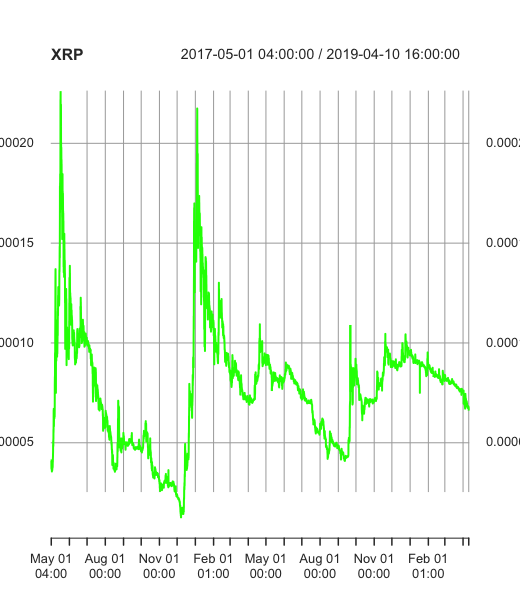
\includegraphics[scale=0.7]{figures/xrp.png}
  \caption{Observed spike in XRP}
  \label{xrp}
\end{figure}

\section{References}
References go here

\end{document}

